\chapter{Aggregation MAC protocol}
\label{aggregation}
%\addtotoc{Aggregation MAC protocol}
\lhead{\emph{Aggregation MAC protocol}}
In the Wireless Sensor Networks with the multi-host topology, the communication between the source node and the destination node can be established through many relay node.
\section{State of the art}
\section{Aggregation MAC protocols}
\subsection{Fixed Aggregation}
\subsubsection{Protocol design}
\label{sec:fa_design}
A simple algorithm of aggregation mechanism which is implemented in the relay node is that each time the relay node receives a data packet from the source nodes, it does not re-transmit immediately to the next relay node or to the destination node. The data packet will be stored in a queue to wait the others data packets. After the $\Delta_{max}$, the relay node aggregates all the data packet with same destination in queue into a aggregated data packet and sends it to the next relay node or to the destination node. With the limitation of resources in sensor node, here is the number of data packet can be stored in the memory, some time the relay node needs to active the process of data aggregation before the $\Delta_{max}$ reached. We define the $\tau_{Q_i}$ is the duration of the $i^{th}$ packet in the queue. The condition of data aggregation is defined in the following equation :
\begin{equation}
\tau_{Q_0} \geq \Delta_{max}\ ||\ qu_{size} = qu_{max}
\label{eq:fa_condition}
\end{equation}
where $\tau_{Q_0}$ is the duration of the $1^{st}$ packet in queue, $\Delta_{max}$ is the limited duration of a packet in queue, $qu_{size}$ is the number of packets in queue and $qu_{max}$ is the limited size of queue depends on the resources of sensor nodes.

The behavior of sensor node which is implemented the Fixed Aggregation MAC protocol is described by the state machine schema in Fig.\ref{fig:fixed_aggregation}.
\begin{figure}[t]
\begin{center}
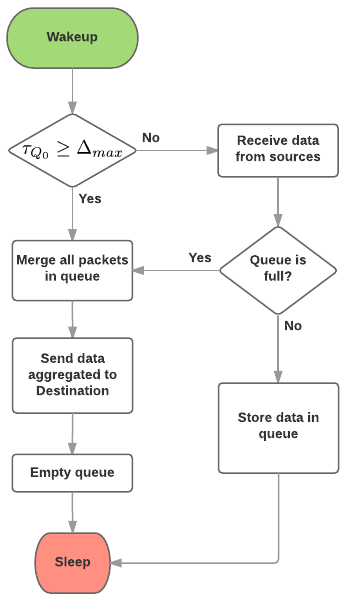
\epsfig{file = ./chapters/chapter5/images/fixed_aggregation.png}
\caption{Behavior of sensor node with Fixed Aggregation MAC protocol.}
\label{fig:fixed_aggregation}
\end{center}
\end{figure}
As other sensor nodes, the relay node uses also the technique duty cycling, it switches between sleep and awake state. But unlike the source or destination nodes, at the beginning of awake state, the relay node will decide to turn on the radio in listening state to receive data from the source nodes or in sending state to transmit the data to the next relay node or to the destination node. To avoid the packet lost caused by the queue is full, the data aggregation is higher priority than receiving data.
\subsubsection{Aggregated packet structure}
As the discussion in the section \ref{sec:fa_design} above, the relay node will aggregate all data packets in the queue and sends a big packet to the destination. A new structure of data packet is proposed in Fig.\ref{fig:aggregated_packet} below.
\begin{figure}[!b]
\begin{center}
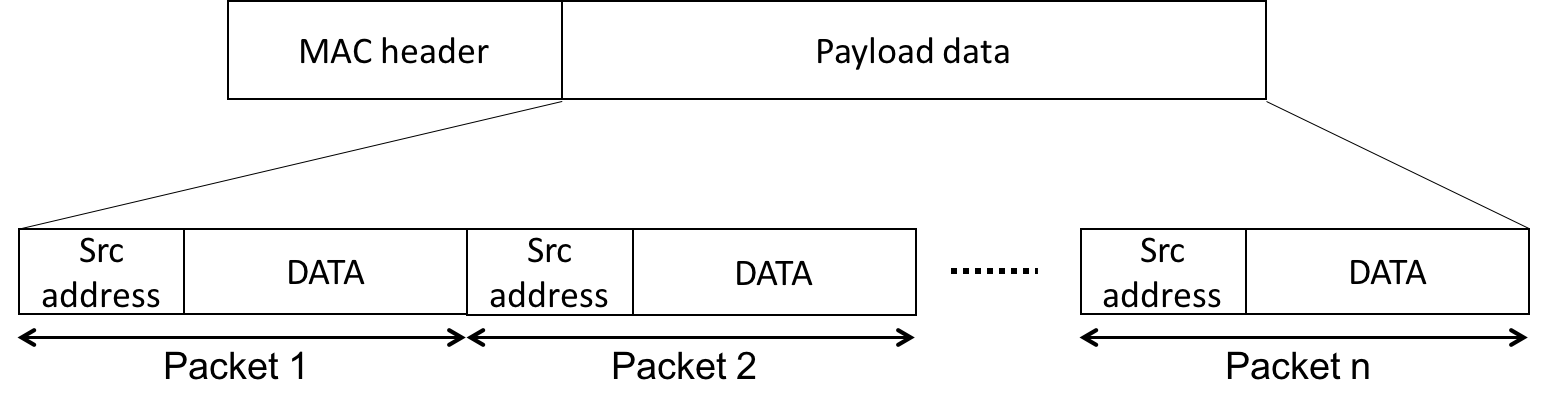
\epsfig{file = ./chapters/chapter5/images/data_structure.png, width=12cm}
\caption{New structure of aggregated packet.}
\label{fig:aggregated_packet}
\end{center}
\end{figure}
With the new structure defined, the size of aggregated data packet is dynamic and can be calculated by the equation following
\begin{equation}
l_{DATA_{agg}} = l_{DATA_{h}} + n(l_{DATA} - l_{DATA_h} + 4)
\label{eq:aggregated_data_length}
\end{equation}
\begin{equation}
t_{DATA_{agg}} = \frac{l_{DATA_{agg}} * 8}{b_{rate}}
\label{eq:aggregated_data_sent_time}
\end{equation}
where $l_{DATA}$ and $l_{DATA_h}$ is the length of data packet and its header, \textit{n} is the number of packet will be aggregated, the condition to use the new structure is \textit{n > 1}, \textit{4} is the number of byte of source address field in header (which is defined in Sec. \ref{sec:fta_frame_structure})

By applying the new structure of data packet and the energy consumption model in duty cycling \ref{sec:fta_energy_model}, the energy saved by sending a new aggregated data packet instead of many single data packet is estimated :
\begin{equation}
\begin{split}
\Delta_E &= n(E_{TX_{DATA}} + E_{RX_{DATA}}) - (E_{TX_{DATA_{agg}}} + E_{RX_{DATA_{agg}}})\\
&= n[4t_{CCA}P_{RX} + (t_{ACK} + t_{DATA})(P_{RX} + P_{TX})] \\
&\quad - [4t_{CCA}P_{RX} + (t_{ACK} + t_{DATA_{agg}})(P_{RX} + P_{TX})] \\
&= (n-1)[4t_{CCA}P_{RX} + t_{ACK}(P_{RX} + P_{TX})] + (P_{RX} + P_{TX})(nt_{DATA} - t_{DATA_{agg}})
\end{split}
\label{eq:aggregated_data_delta_energy}
\end{equation}

From the equations \ref{eq:aggregated_data_length}, \ref{eq:aggregated_data_sent_time} and \ref{eq:aggregated_data_delta_energy} we have :

\begin{equation}
\Delta_E = (n-1)[4t_{CCA}P_{RX} + t_{ACK}(P_{RX} + P_{TX})] + (P_{RX} + P_{TX})\frac{8[(n-1)l_{DATA_{h}} - 4]}{b_{rate}}
\label{eq:aggregated_data_delta_energy}
\end{equation}

The equation \ref{eq:aggregated_data_delta_energy} shows that the more packets aggregated, the more energy saved. But the length of aggregated packet is limited by the hardware of sensor node. So we can not aggregate too much data packets into one big aggregated packet. The number of packets can be aggregated is depend also on the size of data packet which is used in MAC protocol.
\subsection{Dynamic Decision Aggregation}
\subsubsection{Limitation of Fixed Aggregation}
\label{sec:limitation_fa}
In the previous section, we discussed about the Fixed Aggregation mechanism and its advantage in  saving energy consumption. An other advantage of Fixed Aggregation is that the relay nodes do not require any addition information from the source nodes. This feature allows this mechanism is implemented facilely in the MAC protocols. But the fixed waiting duration will increase unnecessarily the delay of data packet in end-to-end communication. This problem is described more detail in the Fig.\ref{fig:fixed_agg_wrong}.
\begin{figure}[!b]
\begin{center}
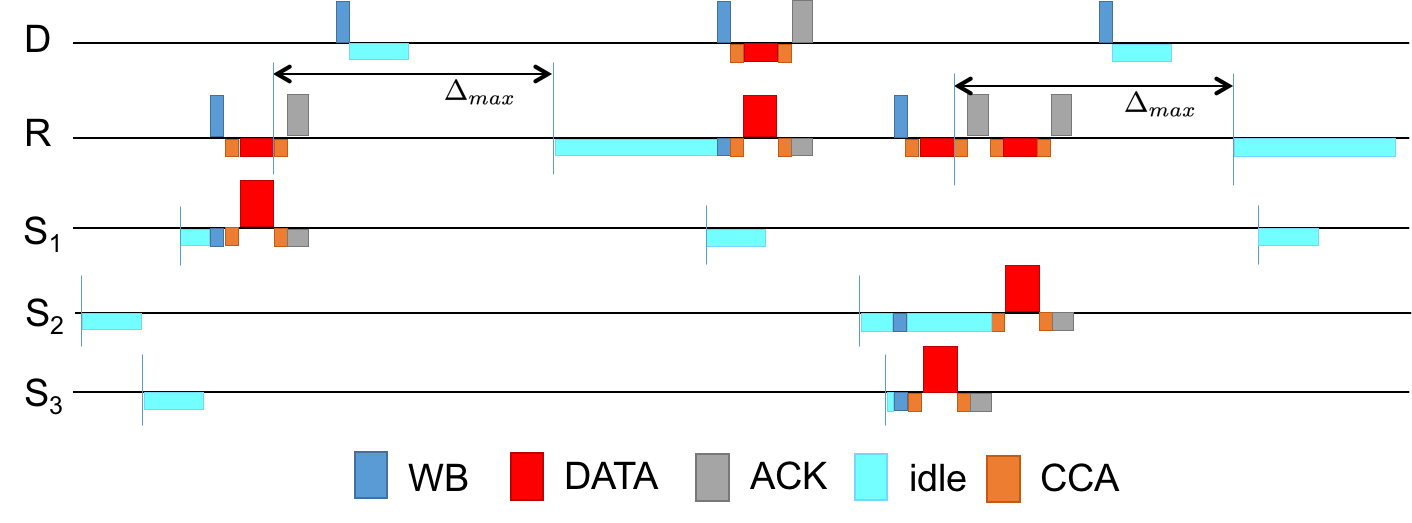
\epsfig{file = ./chapters/chapter5/images/fixed_agg_wrong.png, width=13cm}
\caption{Wasted delay time of Fixed Aggregation.}
\label{fig:fixed_agg_wrong}
\end{center}
\end{figure}
In this example, after receiving data packet from $S_1$, the relay node (\textit{R}) stores this data packet in the queue and makes a schedule to aggregate this packet with the others coming in $\Delta_{max}$ and send the big packet to the destination (\textit{D}). But within the $\Delta_{max}$ second, there is not any packet arrive so the relay node wasted the $\Delta_{max}$s. The problem is also existed in $2^{nd}$ case when the relay node receives the data packets from $S_2$ and $S_3$, it continues wait $\Delta_{max}$s after receiving the $1^{st}$ packet (from $S_3$). This waiting is wasted also.

An other limitation of Fixed Aggregation mechanism is its compatibility of integration with the MAC protocols. In some asynchronized MAC protocols (RICER \cite{ricer}, FTA-MAC \cite{fta-mac}, TAD-MAC \cite{tad-mac}) the communication of sender and receiver is initiated by the receive's WB packet. The waiting duration $\Delta_{max}$ may be caused the missing of destination's WB packet in relay node. In example shown in Fig. \ref{fig:fixed_agg_wrong}, after the waiting duration $\Delta_{max}$, the relay node wakes up and wait the WB packet from the destination, but it already missed the destination's WB packet so it must stay awake to wait the next WB packet. This problem will increase the \textit{idle listing} time and the relay node wastes the energy.
\subsubsection{Dynamic Decision Aggregation}
Dynamic Decision Aggregation is an other approach of data aggregation which avoids the problem of wasted delay time presented in Sec. \ref{sec:limitation_fa}. Unlike Fixed Aggregation mechanism, the relay node does not go to sleep after pushing the data packet into the queue, it estimates the next coming data packets. If there is one or more data packet arrive within $\Delta_{max}$ second, the relay node will wait the coming data packet to aggregate and send to the destination. But note that the duration of staying in queue of a data packet is no longer than $\Delta_{max}$, so the condition of aggregation in Dynamic Decision Aggregation is proposed in the equation following
\begin{equation}
\Delta{t_j} = \widehat{t_j} - t_c\ (\forall{j \neq i})
\label{eq:dda_delta_t_j}
\end{equation}
\begin{equation}
\Delta{t_j} \leq \Delta_{max} - \tau_{Q_0}
\label{eq:dda_condition}
\end{equation}
where \textit{i} index is the index of current source node, $\widehat{t_j}$ is the arrive time of data packet of $j^{th}$ source node, $t_c$ is the current time of system. Because the estimated time $\widehat{t_j}$ is calculated in relay node so it does not require to synchronize the system clock between the sensor nodes.
\begin{figure}[!t]
\begin{center}
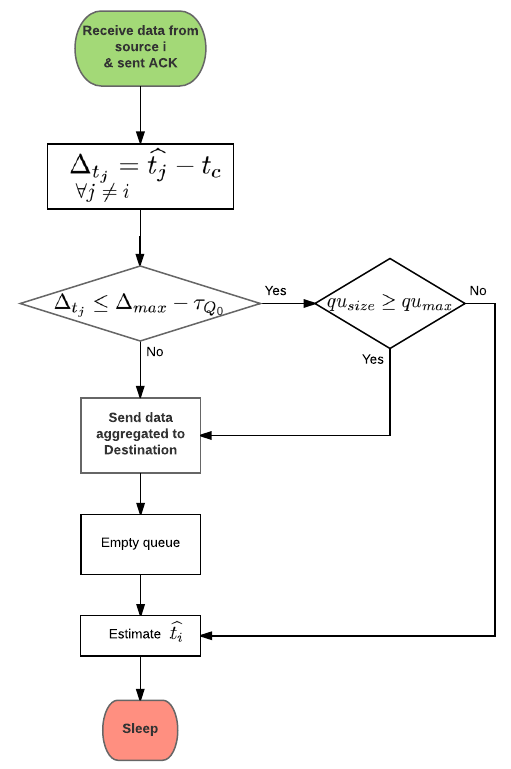
\epsfig{file = ./chapters/chapter5/images/dda.png, width=7cm}
\caption{The state machine of Dynamic Decision Aggregation mechanism.}
\label{fig:dda}
\end{center}
\end{figure}

To estimate the next coming data packet, the method of calculation is depended on the MAC protocols in which the Dynamic Decision Aggregation is implemented. These are some MAC protocols which calculated or allow to calculate easily this value such as PW-MAC \cite{pw-mac}, TAD-MAC, FTA-MAC. Almost MAC protocols do not calculate or have not any additional information which is allow to calculate the next arrival of data packet but we can estimate this value by measuring the traffic. A light weight algorithms is proposed when applying the Dynamic Decision Aggregation in RICER3 (RICER3-DDA protocol). This algorithms is presented in next section.

In considering the problem of wasted delay time presented in Sec. \ref{sec:limitation_fa}, this problem will be resolved by applying the new condition of aggregation in the equation \ref{eq:dda_condition} and \ref{eq:dda_delta_t_j} which is shown in Fig.\ref{fig:dda_2}.
\begin{figure}[!b]
\begin{center}
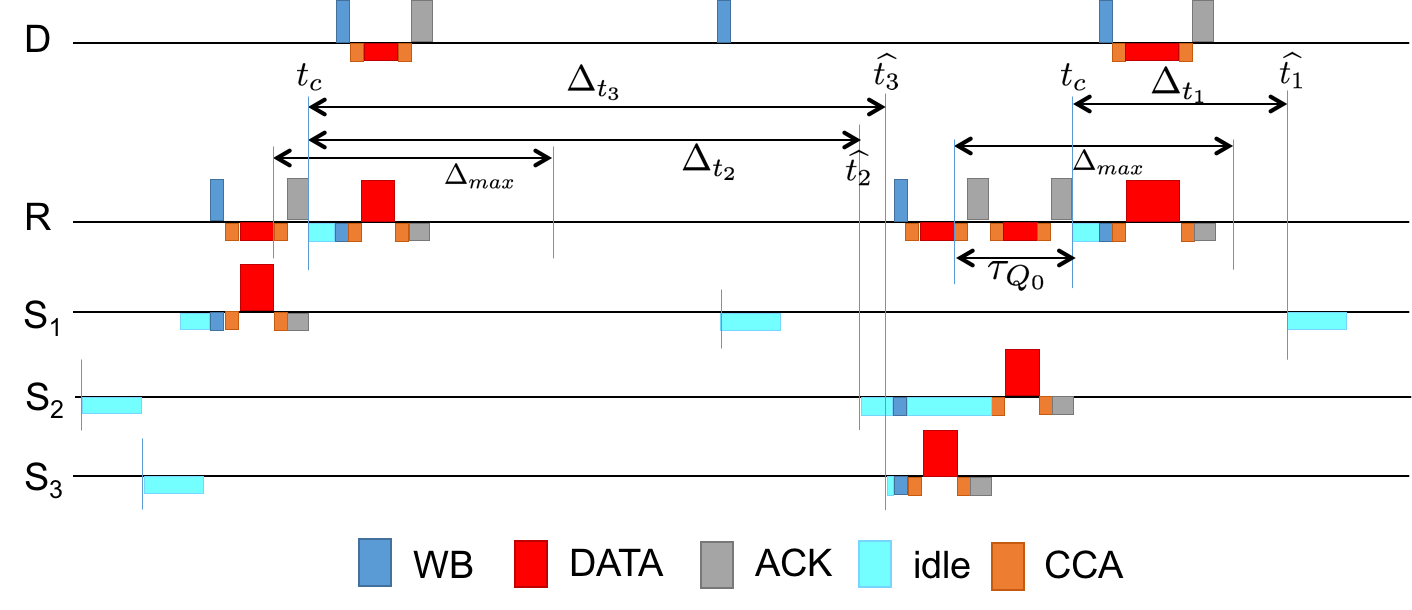
\epsfig{file = ./chapters/chapter5/images/dda_2.png, width=13cm}
\caption{Solution of wasted delay time in Dynamic Decision Aggregation mechanism.}
\label{fig:dda_2}
\end{center}
\end{figure}
Precisely, at the $1^{st}$ case, after sending the ACK packet back to $S_1$, the relay node calculates these values $\Delta_{t_2}$ \& $\Delta_{t_3}$ to make the decision of aggregation. The next arrival of data packets from $S_2$ \& $S_3$ is so long to make the aggregation so the relay node does not go to sleep, it stays awake to wait the WB from the destination and transmits the data packet to destination. In the $2^{nd}$ case, we suppose the MAC protocol already has mechanism to solve the problem of data conflict, so the process of aggregation will be started after sending the ACK packet back to $S_2$, when all communications between the relay node and the source nodes are finished. This applying will not change the algorithm of MAC protocol. 
\section{Implementation and Evaluation}
To evaluate the performance of Fixed Aggregation and Dynamic Decision Aggregation, we implement them in the exist MAC protocols like RICER3, FTA-MAC.
\subsection{Implementation of the aggregation MAC protocols in RICER3}
\subsubsection{RICER3 Fixed Aggregation (RICER3-FA)}
The implementation of Fixed Aggregation in RICER3 is applied on the relay node.
The basic behavior of RICER3-FA is described in Fig. \ref{fig:ricer_fa}. As describing in Sec. \ref{sec:fa_design}, the implementation is applied on the relay node. In each cycling, the Fixed Aggregation mechanism is executed at the end of the communication between relay node (\textit{R}) and the senders ($S_1$, $S_2$, $S_3$) to verify the aggregation condition in Eq. \ref{eq:fa_condition}. If the condition is satisfied, the relay node will stay awake to wait the \textit{WB} from the receiver and sends the aggregated data packet to the receiver. Otherwise, it go to sleep and finish a duty cycling. An additional timer is used in the relay node to compute the queuing time of the first packet. \ref{eq:dda_delta_t_j}
\begin{figure}[!b]
\begin{center}
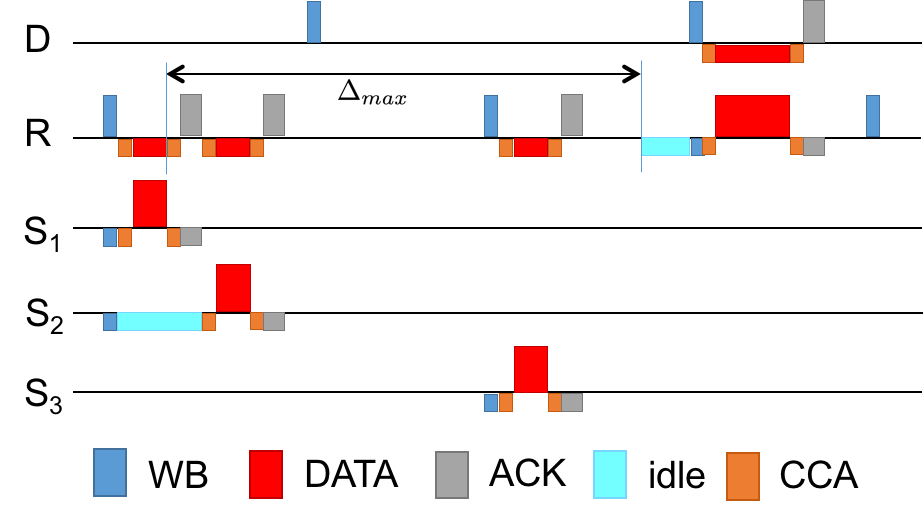
\epsfig{file = ./chapters/chapter5/images/ricer_agg.png, width=12cm}
\caption{Basic behavior of RICER with Fixed Aggregation.}
\label{fig:ricer_fa}
\end{center}
\end{figure}
\subsection{Evaluation}
\subsubsection{Simulation parameters}
\subsubsection{Results}